\documentclass[17pt]{beamer}

\usepackage[utf8]{inputenc}
\usepackage{listings}
\usepackage{tikz}
\usetikzlibrary{positioning}
\usetikzlibrary{arrows.meta}
\usepackage{pgfplots}
\pgfplotsset{compat=1.16}
\usepackage{inconsolata}

% output configuration
\usepackage{pgfpages}
%\setbeameroption{show notes on second screen=left}
\hypersetup{pdfpagemode=FullScreen}

% presentation themeing
\usetheme{Singapore}
\beamertemplatenavigationsymbolsempty
\setbeamertemplate{bibliography item}{\insertbiblabel}

% Julia listings definition
% Definition based on https://tex.stackexchange.com/a/212794/149437
\lstdefinelanguage{Julia}
  {otherkeywords={::},
   keywords=[1]{::,abstract,break,case,catch,const,continue,do,else,elseif,
      end,export,for,function,immutable,import,importall,if,in,
      macro,module,otherwise,quote,return,switch,try,type,typealias,
      using,while,where},
   keywords=[2]{false,true},
   sensitive=true,
   alsoother={$},
   morecomment=[l]\#,
   morecomment=[n]{\#=}{=\#},
   morestring=[s]{"}{"},
   morestring=[m]{'}{'},
}[keywords,comments,strings]

\lstset{
	language         =Julia,
	basicstyle       =\ttfamily\footnotesize,
	columns          =fixed,
	numbers          =left,
	keywordstyle     ={[1]\bfseries\color{black}},
	keywordstyle     ={[2]\color{blue}},
	stringstyle      =\color{red},
	commentstyle     =\color{gray},
	showstringspaces =false,
	mathescape
}


\title[JuliaPetra]{Obtaining Performance from a Julia-Implementation of Trilinos Data Libraries}
\author{Neil Lindquist}
\institute{Saint John's University, Minnesota}
\date[SIAM CSE19]{\small SIAM Conference on Computational Science and Engineering\\February 27th 2019}


\begin{document}
\frame{\titlepage}
\begin{frame}
	\frametitle{Julia}
	\nocite{Bezanson:2017:FreshApproach}
	\begin{itemize}
		\item High Level
		\item Compiles to efficient machine code
	\end{itemize}
	%TODO consider if Wilkins prize should be mentioned
	%TODO should LLVM be mentioned?
	\note{
		high level, dynamic language
		
		can perform on par with C
		
		investigating whether Julia is usable for distributed, high performance codes
	}
\end{frame}

\begin{frame}
	\frametitle{Petra Object Model}
	\nocite{Heroux:2005:Trilinos}
	\begin{itemize}
		\item Underlying data libraries for Trilinos
		\item Family of sparse linear algebra frameworks
		\item 3 existing implementations
	\end{itemize}
	\note{
		Trilinos uses a family of libraries know as the Petra Object Model for its core data represetation
		
		These libraries are basic frameworks for sparse linear algebra
		
		3 implementations
		\begin{itemize}
			\item Epetra - original, portable version C++
			\item Tpetra - newer, uses more advanced C++ features
			\item Jpetra - experiemental, pure java version
		\end{itemize}
	}
\end{frame}
\begin{frame}
	\frametitle{Petra Organization}
	\nocite{Github:MPI}
	\centering
	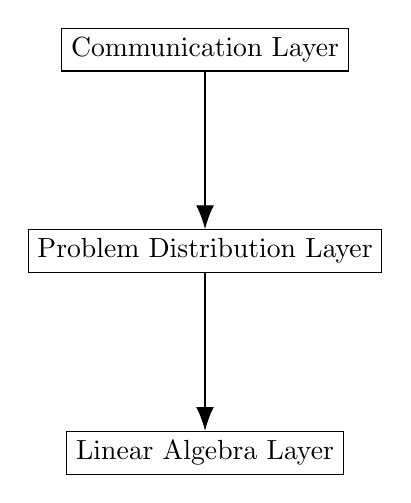
\begin{tikzpicture}
		\node[rectangle, draw=black] (CommLayer) {Communication Layer};
		\pause
		\node[rectangle, draw=black] (DistLayer) [below=2cm of CommLayer] {Problem Distribution Layer};
		\draw[-{Latex[length=3mm]}] (CommLayer.south) -- (DistLayer);
		\pause
		\node[rectangle, draw=black] (LALayer) [below=2cm of DistLayer] {Linear Algebra Layer};
		\draw[-{Latex[length=3mm]}] (DistLayer.south) -- (LALayer);
	\end{tikzpicture}
	\note<1>{
		Communication layer handles the movement of data between processes
		\begin{itemize}
			\item Can be implemented with any Single-Program-Multiple-Data parallel system
			\item There are serial and MPI implementations
		\end{itemize}
	}
	\note<2>{
		Distribution layer managed how the parts of the problem are distributed
		
		This layer isn't extended by the user %Note totally true, DistObject is here
	}
	\note<3>{
		Linear Algebra layer provides the interfaces for vector and linear transformation objects
	}
\end{frame}
\begin{frame}[fragile]
	\frametitle{JuliaPetra Example I}
	\begin{lstlisting}
function powerMethod(A::RowMatrix{Data},
        tol::Data) where Data
    blockmap = getRowMap(A)
    q = DenseMultiVector{Data}(blockmap, 1)
    z = DenseMultiVector{Data}(blockmap, 1)
    randn!(z.data)
    r = DenseMultiVector{Data}(blockmap, 1)
	\end{lstlisting}
	\note{
		Sample implementation of the power method for finding eigenvalues.
		
		This is the method setup
		
		Note that the data type used by the vectors is just listed as ``Data''
	}
\end{frame}
\begin{frame}[fragile]
	\frametitle{JuliaPetra Example II}
	\begin{lstlisting}[firstnumber=8]
    while true
        normz = norm2(z)
        @. q = z/normz
        apply!(z, A, q)
        $\lambda$ = q$\,\mathtt{\boldsymbol{\cdot}}\,$z  # = dot(q, z)
        @. r = z - $\lambda$*q
        if norm2(r)[1] < tol
            return $\lambda$
        end
    end
end
	\end{lstlisting}
	\note{
		This is the main loop of the method
		
		``apply!'' is the matrix vector product
		\begin{itemize}
			\item exclemation indicates z is mutated
		\end{itemize}
		
		unicode support
		\begin{itemize}
			\item Julia editors support latex-like abbreviations
		\end{itemize}
		
		``@.'' is the broadcast operator
		\begin{itemize}
			\item Should be a single loop, without allocating a vector
			\item multivector scalars
		\end{itemize}
	}
\end{frame}
\begin{frame}
	\frametitle{Performance Comparison}
	\nocite{Github:DA, Gu:2000:PowerMethod}
	\centering
	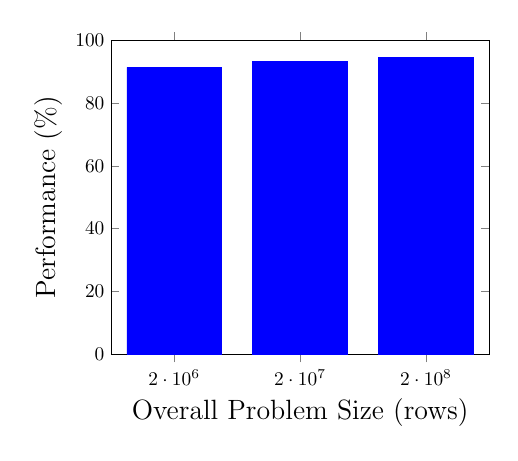
\begin{tikzpicture}[scale=0.7]
		\begin{axis}[
			xlabel = {\Large Overall Problem Size (rows)},
			xtick = {6,7,8},
			xticklabels = {\(2\cdot10^6\), \(2\cdot10^7\), \(2\cdot10^8\)},
			xmin = 5.5,
			xmax = 8.5,
			ybar,
			bar width = 0.75,
			ylabel = {\Large Performance (\%)},
			ymin  = 0,
			ymax  = 100,
			yticklabel style={/pgf/number format/fixed},
			]
			\addplot[blue,fill=blue] coordinates{(6, 91.362)(7,93.146)(8,94.536)};
		\end{axis}
	\end{tikzpicture}
	
	20 CPU processes on a 20 core node.
	\note{
		Power method for finding eigenvalues
		
		Relative to Epetra, JuliaPetra is slightly slower, but still close.
		\begin{itemize}
			\item JuliaPetra is between 90- and 95\% of Epetra
			\item larger problems are closer
		\end{itemize}
		
		DistributedArrays was significantly slower
	}
\end{frame}
\begin{frame}
	\frametitle{Performance Comparison}
	\centering
	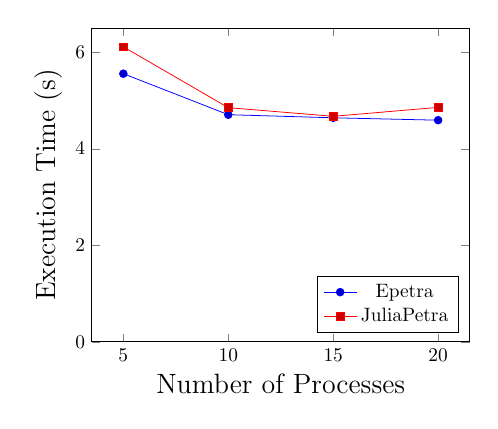
\begin{tikzpicture}[scale=0.7]
		\begin{axis}[
			xlabel = {\Large Number of Processes},
			ylabel = {\Large Execution Time (s)},
			ymin = 0,
			ymax = 6.5,
			legend pos = south east
		]
			\addplot coordinates{(5, 5.554918) (10, 4.705534) (15, 4.64124) (20, 4.591788)};
			\addlegendentry{Epetra}
			\addplot coordinates{(5, 6.110807973) (10, 4.851059517) (15, 4.67226152) (20, 4.856775282)};
			\addlegendentry{JuliaPetra}
		\end{axis}
	\end{tikzpicture}
	
	\(10^7\) rows on a 20 core node.
	\note{
		Comparison for varying numbers of processes.
		
		JuliaPetra has something weird going on, since perfomance slightly drops when every core is used.  Epetra doesn't have this problem.
	}
\end{frame}
\begin{frame}
	\frametitle{Optimizing JuliaPetra}
	\begin{itemize}
		\item Requires disabling high level features
		\begin{itemize}
			\item Dynamic Typing
			\item Garbage Collection
			\item Bounds Checks
		\end{itemize}
	\end{itemize}
	\note{
		Because Julia is a high level language, critical sections need to remove some high level features to perform efficiently.
		
		There are 3 main sets of high level features that I needed to work around
		\begin{itemize}
			\item Dynamic typing
			\item Garbage collection
			\item Bounds checks
		\end{itemize}
	}
\end{frame}
\begin{frame}
	\frametitle{Type Stability}
	\framesubtitle{Optimizing JuliaPetra}
	\begin{itemize}
		\item type annotations are optional
		\item types inferred \(\implies\) ``Type Stable''
		\item allows inlining
	\end{itemize}
	\note{
		compile deducing types important for performance
		
		called type stability.
		
		allows static dispatch and inlining
		\begin{itemize}
			\item basic operators implemented as function calls
		\end{itemize}
		
		each method compiled with each concrete signature
	}
\end{frame}
\begin{frame}
	\frametitle{Type Stability Tools}
	\framesubtitle{Optimizing JuliaPetra}
	\nocite{Github:TypeStability.jl}
	\begin{itemize}
		\item \texttt{code\_warntype} - view inferred types
		\item TypeStability.jl - Automated checking
	\end{itemize}
	\note{
		tools to ensure code is type stable are crucial
		
		code\_warntype is a built in function to manually inspected the results of type inferencing and inlining.
		
		However, checking that a function behaves for different sets of arguments is very tedious.
		
		To automate type stability checks, I created a basic package, TypeStability.jl.
	}
\end{frame}
\begin{frame}
	\frametitle{Reducing Garbage Collection}
	\framesubtitle{Optimizing JuliaPetra}
	\begin{itemize}
		\item Garbage collection is automatic
		\item \texttt{Ptr} type doesn't need garbage collection
	\end{itemize}
	\note{
		Garbage collection is automatic
		
		Only immutable objects that don't reference heap allocated objects can be allocated with the stack for cheap deallocation.
		
		Matrix vector product requires heavy use of array views.
		
		Used a pointer type from the C interface to prevent heap allocating views.
		
		This trick only works were original array is safe from garbage collection
	}
\end{frame}
\begin{frame}
	\frametitle{Bounds Checks}
	\framesubtitle{Optimizing JuliaPetra}
	\begin{itemize}
		\item Julia checks bounds automatically
		\item \texttt{@inbounds} macro skips bounds checks
	\end{itemize}
	\note{
		Julia checks boundaries by default
		
		Want to eliminate those checks when known to be unnecessary
		
		Julia has a \texttt{inbounds} macro to indicate that bounds checks aren't needed
		\begin{itemize}
			\item Only honored when bound check is inlined into the calling method.
		\end{itemize}
	}
\end{frame}
\begin{frame}
	\frametitle{Conclusion}
	\begin{itemize}
		\item promising, high level language
		\item clean APIs
		\item high performance
	\end{itemize}
	\note{
		Julia is fast and high level
		
		Julia allows for elegant math APIs due to type inferencing and broadcast operator
		
		JuliaPetra matches Epetra performance
		
		Julia can be optimized by eliminating the overhead of some high level features
		
		These factors make Julia a good candiate for large scale, high performance codes.
	}
\end{frame}
\begin{frame}[fragile]
	\frametitle{Try It}
	\small
	\url{github.com/collegeville/JuliaPetra.jl}
	\bigskip
	\begin{lstlisting}[numbers=none,basicstyle=\ttfamily]
Pkg.add("JuliaPetra")
	\end{lstlisting}
\end{frame}
\begin{frame}[allowframebreaks]
	\frametitle{References}

	\bibliographystyle{siam}
	\small\bibliography{bibliography}

\end{frame}
\end{document}
